% 1074(본책 149쪽) — 함수 f: X→X 대응 그림. X={1,2,3}, 1→3, 2→1, 3→2(답지 99쪽 풀이와 대조). 스캔 그림이라 TikZ 로 다시 그림.
% 라벨은 원문 그대로 X·X·f·원소만.
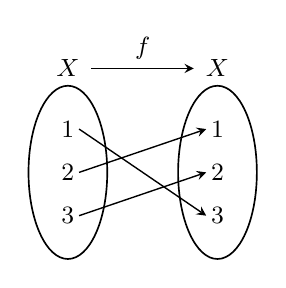
\begin{tikzpicture}[line width=0.5pt, every node/.style={font=\small}]
  \draw[line width=0.6pt] (0.00,0.00) ellipse (0.5 and 1.10);
  \draw[line width=0.6pt] (1.90,0.00) ellipse (0.5 and 1.10);
  \node at (0.00,1.32) {$X$};
  \node at (1.90,1.32) {$X$};
  \draw[->, >=stealth] (0.30,1.32) -- (1.60,1.32);
  \node at (0.95,1.58) {$f$};
  \node[inner sep=1.5pt] (x0) at (0.00,0.55) {$1$};
  \node[inner sep=1.5pt] (x1) at (0.00,0.00) {$2$};
  \node[inner sep=1.5pt] (x2) at (0.00,-0.55) {$3$};
  \node[inner sep=1.5pt] (y0) at (1.90,0.55) {$1$};
  \node[inner sep=1.5pt] (y1) at (1.90,0.00) {$2$};
  \node[inner sep=1.5pt] (y2) at (1.90,-0.55) {$3$};
  \draw[->, >=stealth] (x0.east) -- (y2.west);
  \draw[->, >=stealth] (x1.east) -- (y0.west);
  \draw[->, >=stealth] (x2.east) -- (y1.west);
\end{tikzpicture}
